\begin{figure}
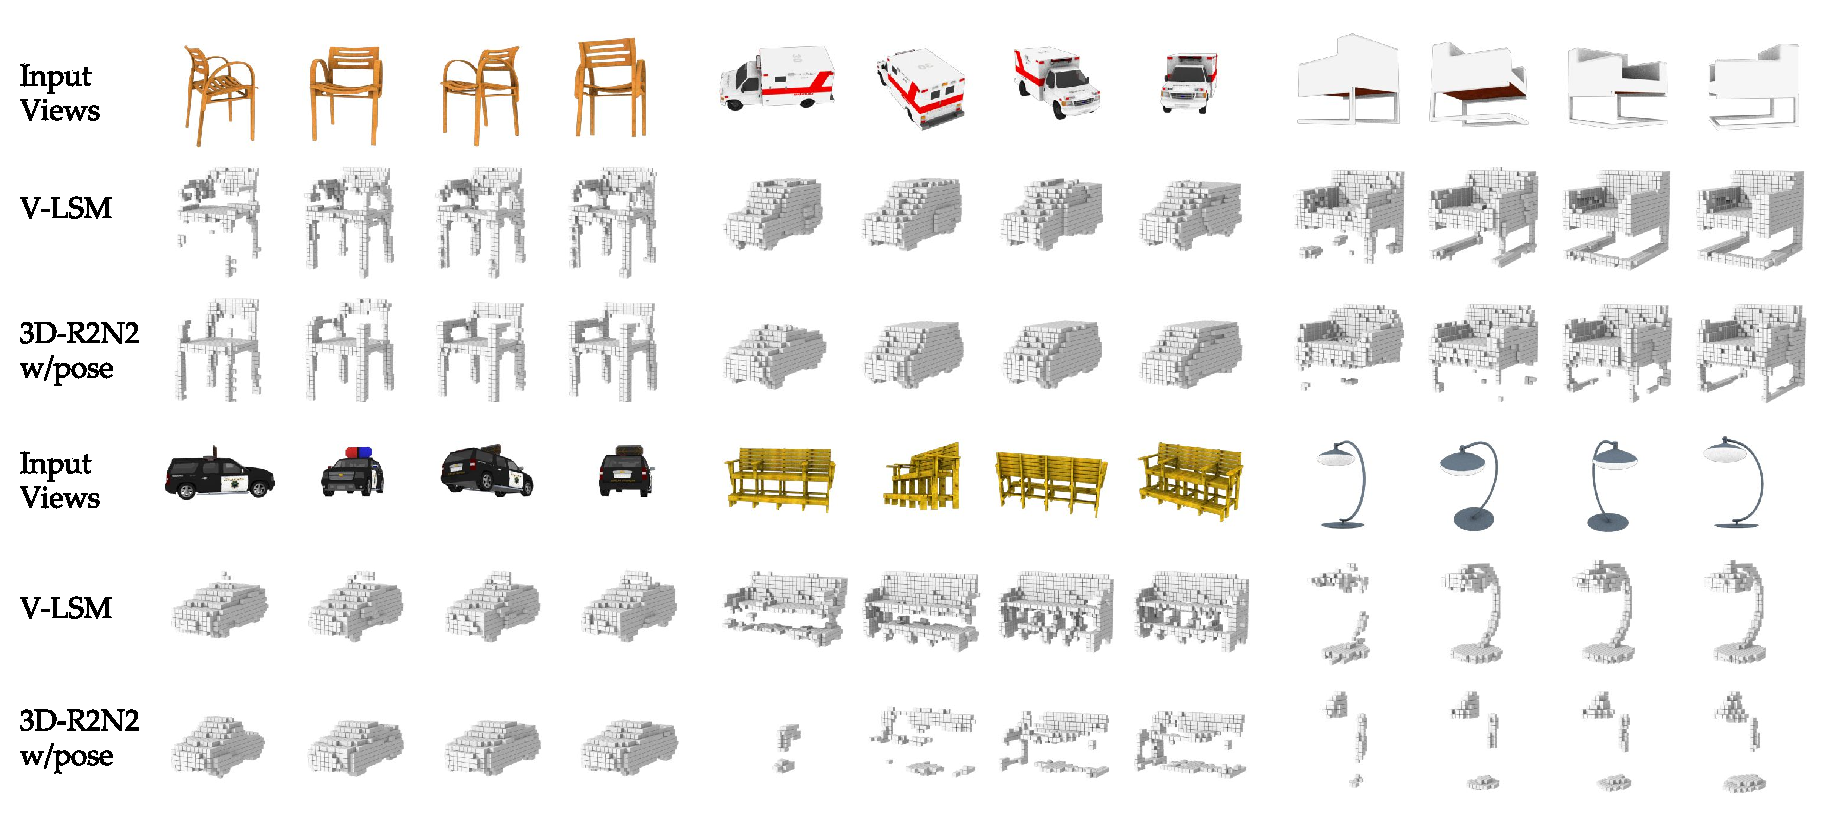
\includegraphics[width=\linewidth]{figures/voxel_results.pdf}
\caption{Voxel grids produced by V-LSM for example image sequences alongside a learning based baseline which uses pose information in a fully connected manner. V-LSM produces geometrically meaningful reconstructions (\eg the curved arm rests instead of perpendicular ones (in R2N2) in the chair on the top left and the siren lights on top of the police car) instead of relying on purely semantic cues. More visualizations in supplementary material.}
\figlabel{voxel_results}
\end{figure}